\documentclass{beamer}

\usepackage{Vor2018glærur}

\title{Tölvunarfræði 2}
\subtitle{Vika 8}

\begin{document}

\begin{frame}
	\titlepage
\end{frame}

\section{Inngangur}

\section{Nafnatöflur}

\begin{frame}{Nafnatöflur}
	\begin{columns}
		\column{0.5\textwidth}
		\begin{itemize}
			\item Nafnatafla \eng{symbol table} er mjög almenn hugræn gagnagrind
			\item Snýst um að tengja saman lykla (e. \emph{keys}) og gildi (e. \emph{values})
			      \begin{itemize}
				      \item ``Hvert er gildið fyrir þennan lykil?''
			      \end{itemize}
			\item Þurfum að leysa leitarvandamál
		\end{itemize}
		\column{0.5\textwidth}
		\begin{center}
			DNS tafla
			\begin{tabular}{cc}
				\toprule
				Lykill   & Gildi           \\
				\midrule
				mbl.is   & 92.43.192.110   \\
				visir.is & 82.221.81.10    \\
				hi.is    & 130.208.165.207 \\
				ru.is    & 52.48.55.82     \\
				\bottomrule
			\end{tabular}
		\end{center}
	\end{columns}
\end{frame}

\begin{frame}{Hagnýtingar}
    \begin{center}
        Leit eftir lykli kemur \emph{víða} við
        \vspace{0.5cm}
        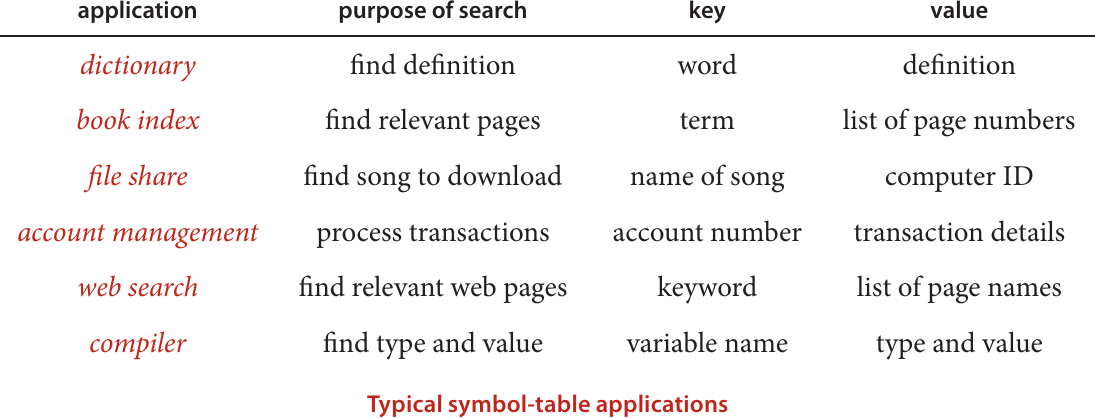
\includegraphics[width=\textwidth]{symbol-table-applications}
        \vspace{0.5cm}
        Algorithms, 4th edition, bls. 362
    \end{center}
\end{frame}

\begin{frame}{API}
	Möguleg skil fyrir nafnatöflu:
	\vspace{0.5cm}
	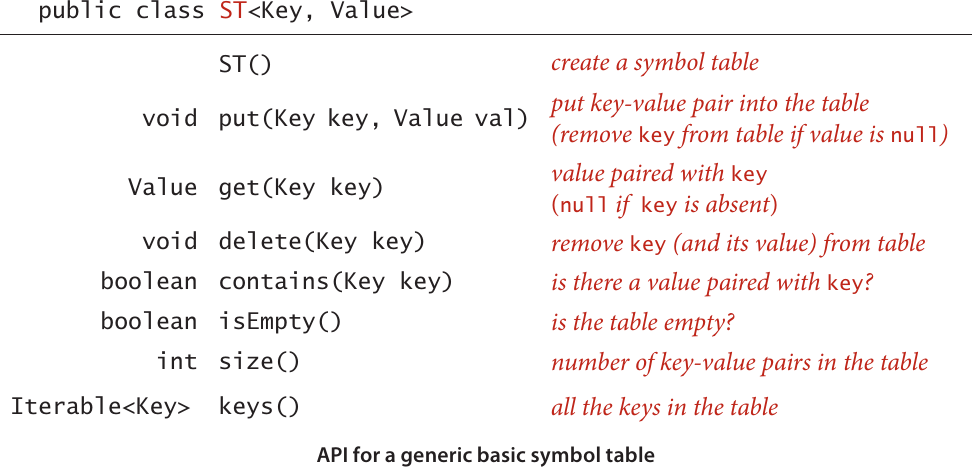
\includegraphics[width=0.9\textwidth]{symbol-table-api}
	Algorithms, 4th edition, bls. 363
\end{frame}

\begin{frame}{Gögnin í nafnatöflu}
	\begin{itemize}
		\item Lyklar og gildi þurfa ekki að vera af sömu gagnagerð
		\item Í okkar útfærslum:
		      \begin{itemize}
			      \item Lyklar mega ekki vera \texttt{null}
			            \begin{itemize}
				            \item Einfaldar forritun
			            \end{itemize}
			      \item Gildi mega ekki vera \texttt{null} heldur
			            \begin{itemize}
				            \item Látum \texttt{get(key)} sem skilar \texttt{null} tákna að ekkert gildi sé venslað við \texttt{key}
				            \item Látum \texttt{put(key, null)} eyða staki úr töflunni
			            \end{itemize}
		      \end{itemize}
		\item Almennt ráðlagt: Nota óbreytanlega \eng{immutable} lykla
		      \begin{itemize}
			      \item Gott: \texttt{Integer}, \texttt{String}, \texttt{Double},\ldots
			      \item Slæmt: T.d. fylki
		      \end{itemize}
	\end{itemize}
\end{frame}

\begin{frame}{Útfærsla á nafnatöflu}
	\begin{itemize}
		\item Við gætum sett gögnin okkar í óraðað fylki eða eintengdan lista
		\item Skoðum \href{http://algs4.cs.princeton.edu/code/edu/princeton/cs/algs4/SequentialSearchST.java.html}{SequentialSearchST.java}
		\item Vandamál: Línulegur innsetningartími, línulegur uppflettingartími
		      \begin{itemize}
			      \item Af hverju ekki fastur innsetningartími?
		      \end{itemize}
	\end{itemize}
\end{frame}

\begin{frame}{Betrumbætur}
	\begin{itemize}
		\item Getum notað öflugri aðferðir ef við getum gert ráð fyrir meiru um lyklana
		\item Skoðum núna: lykla sem eru samanburðarhæfir (sjá \texttt{Comparable})
		\item Gerir mögulegt að geyma stökin í röðuðu fylki
		\item Fjölgar aðferðunum sem okkur gætu staðið til boða
	\end{itemize}
\end{frame}

\imageslide[1.2cm]{symbol-table-ordered-api}

\section{Helmingunarleit}

\begin{frame}{Helmingunarleit}
	\begin{itemize}
		\item Getum gert betur en  í röðuðum fylkjum, hugmyndin er:
		      \begin{itemize}
			      \item Berum ``miðju'' leitarbilsins saman við leitarstakið
			      \item Sé miðjan stærri en leitarstakið vitum við að stakið er ekki að finna í stærri helming leitarbilsins (og öfugt)
			      \item Notum helmingunarleit endurkvæmt á þann helming leitarbilsins sem eftir er
		      \end{itemize}
		\item Leitaraðferðin er kölluð helmingunarleit \eng{binary search} því hún helmingar stærð leitarbilsins í hverri ítrun
		\item Grundvallaraðferðafræði sem kemur víða við!
		\item Skoðum \href{http://algs4.cs.princeton.edu/code/edu/princeton/cs/algs4/BinarySearchST.java.html}{BinarySearchST.java} vandlega
	\end{itemize}
\end{frame}

\begin{frame}{Endurkvæm helmingunarleit}
	\begin{center}
		Möguleg endurkvæm útfærsla á helmingunarleit:

		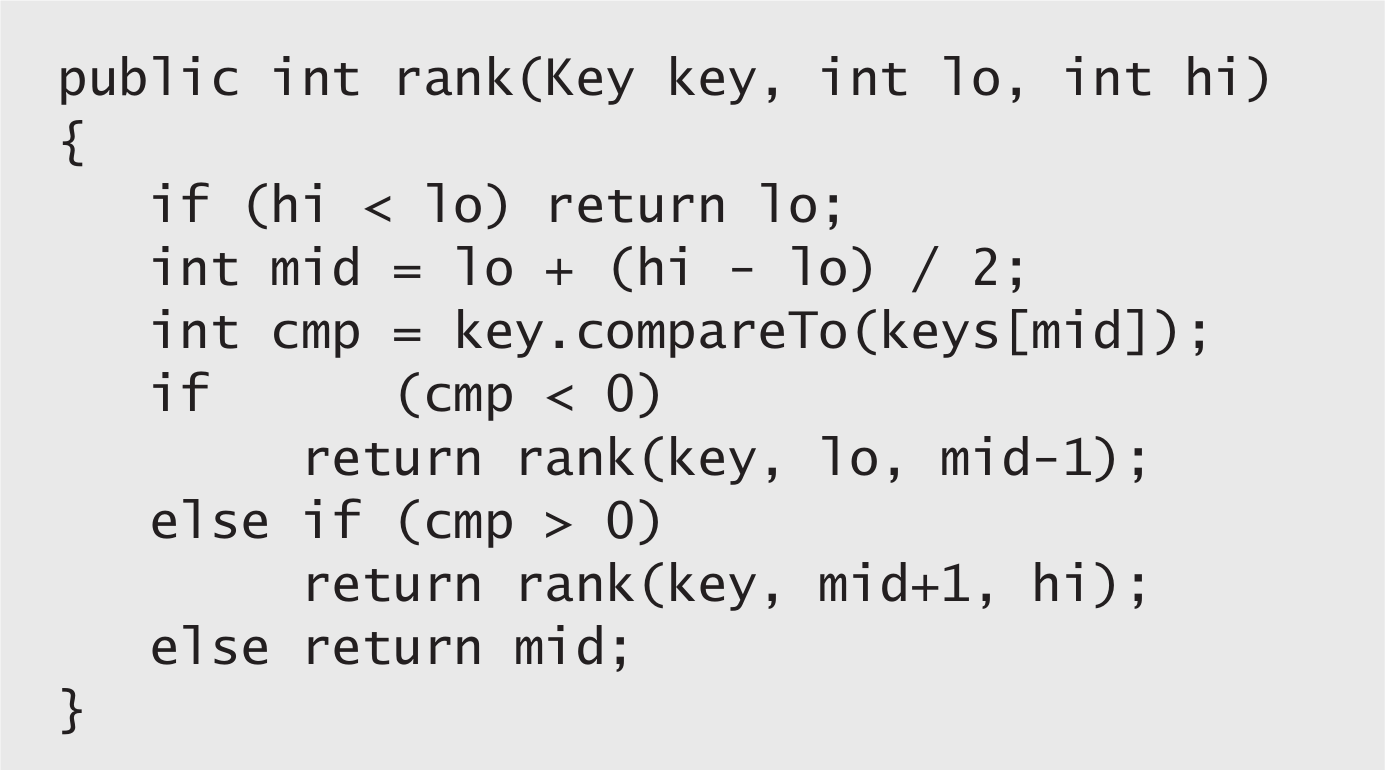
\includegraphics[width=0.7\textwidth]{binary-search-algs4-380}
	\end{center}
	Algorithms, 4th edition, bls. 380
\end{frame}

\begin{frame}{Tími}
	\begin{columns}
		\column{0.6\textwidth}
		\begin{itemize}
			\item Getum lýst fjölda samanburða í helmingunarleit í $N$ staka fylki með rakningarvenslum:
			      \begin{itemize}
				      \item $C(0) = 0$, $C(1) = 1$ , $C(N) = C(\lfloor N/2 \rfloor)+1$
				      \item Fáum $C(N) \sim \log N$
			      \end{itemize}
			\item Útfærslan á nafnatöflunni í \texttt{BinarySearchST.java} leyfir skilvirkar uppflettingar (logratími)
			\item Innsetningar og eyðingar krefjast hins vegar enn línulegs tíma
		\end{itemize}
		\column{0.4\textwidth}
		\begin{center}
			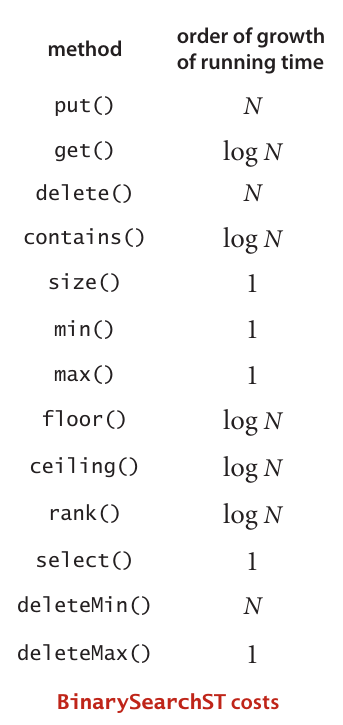
\includegraphics[width=0.7\linewidth]{binary-search-times-table}

			Algorithms, bls. 384
		\end{center}
	\end{columns}
\end{frame}

\begin{frame}{Innsetning í raðaða töflu}
	\begin{center}
		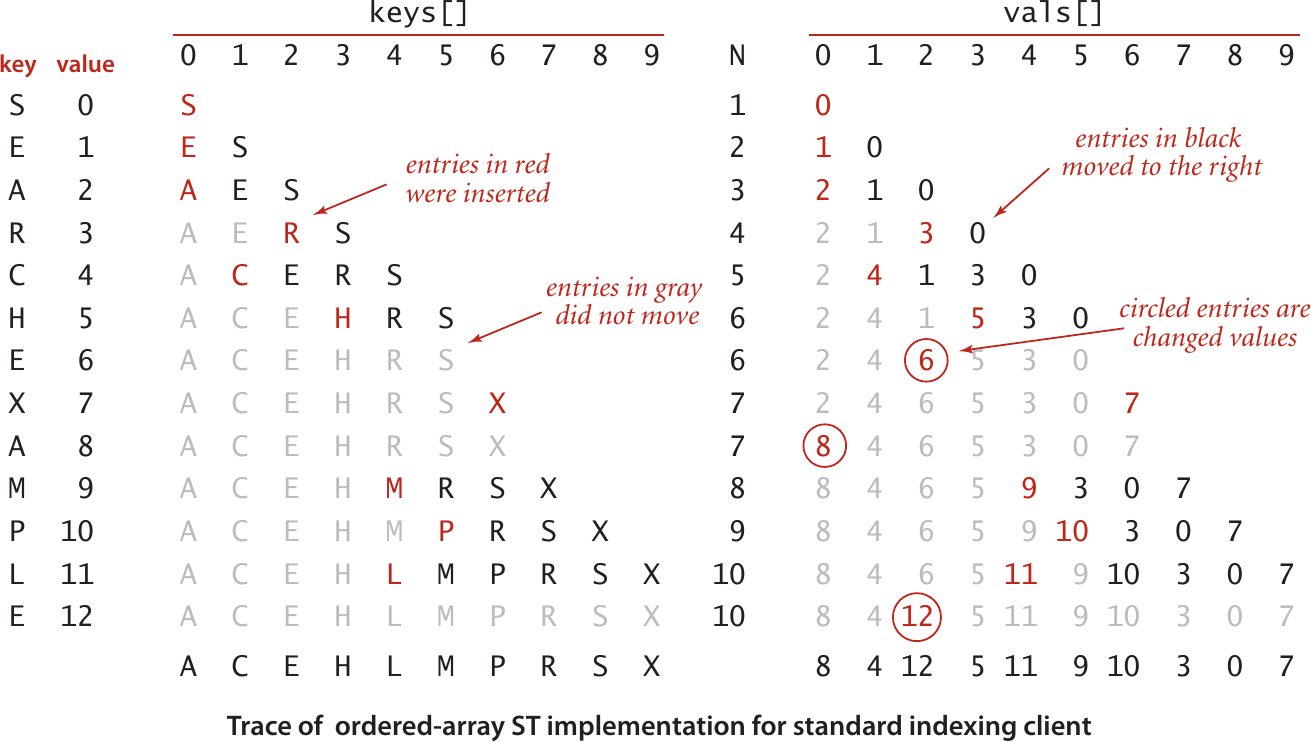
\includegraphics[width=0.9\textwidth]{symbol-table-ordered-insertion}

		Algorithms, 4th edition, bls. 378
	\end{center}


\end{frame}

\section{Tvíleitartré}

\begin{frame}{Tvíleitartré}
	\begin{itemize}
		\item Við getum auðveldað helmingunarleit með því að geyma gögnin í tvíundartré \eng{binary tree}
		      \begin{itemize}
			      \item Í þetta skiptið - táknað með hnútum og bendum, líkt og við höfum gert þegar við höfum útfært eintengda lista
		      \end{itemize}
		\item Til að útfæra nafnatöflu látum við hnúta innihalda samanburðarhæfan lykil, notum uppbyggingu trésins til að auðvelda leitina
		      \begin{itemize}
			      \item Látum vinstra barn hvers hnúts hafa minni lykil en hnúturinn, hægra barnið stærri lykil
		      \end{itemize}
		\item Köllum þessi tvíundartré tvíleitartré \eng{binary search tree}
		\item Skoðum nafnatöflu útfærða með tvíleitartré, \href{http://algs4.cs.princeton.edu/code/edu/princeton/cs/algs4/BST.java.html}{BST.java}
	\end{itemize}
\end{frame}

\begin{frame}{Aðgerðir á tvíleitartré}
	\begin{itemize}
		\item Til að uppfylla lágmarkssskil fyrir nafnatöflu þurfum við að geta:
		      \begin{itemize}
			      \item Leitað eftir lykli (\texttt{get})
			            \begin{itemize}
				            \item Berum leitarlykilinn saman við lykil hvers hnúts
				            \item Förum í vinstra eða hægra undirtré eftir hvern samanburð
				            \item Hættum þegar lykillinn finnst eða þegar við finnum \texttt{null}
			            \end{itemize}
			      \item Sett inn gögn (\texttt{put})
			            \begin{itemize}
				            \item Svipað og leit, en þegar við finnum \texttt{null} setjum við stakið inn
			            \end{itemize}
		      \end{itemize}
	\end{itemize}
\end{frame}

\imageslide{AlgsSlides/bst-intro}

\imageslide{AlgsSlides/bst-search}

\imageslide{AlgsSlides/bst-insert}

\imageslide{AlgsSlides/bst-shapes}

\begin{frame}{Erfiðleikar í nafnatöflum}
	\begin{itemize}
		\item Raunveruleg notkun á nafnatöflum gerir greiningu erfiða
		      \begin{itemize}
			      \item Uppfletting og innsetning gerast sitt á hvað
			      \item Fjöldi lykla getur verið mjög stór
			      \item Tíðni uppflettinga og innsetninga eru illfyrirsjáanleg en ekki slembin
		      \end{itemize}
		\item Þurfum að ákveða útfærslu vandlega
	\end{itemize}
\end{frame}

\begin{frame}{Þessi glærupakki}
    Kóða fyrir algs4 reiknirit má finna á \url{http://algs4.cs.princeton.edu/code/}
    
    Gráar glærur eru úr \url{https://algs4.cs.princeton.edu/lectures/32BinarySearchTrees.pdf}
\end{frame}

\begin{frame}{Næst}

    \href{https://piazza.com/class/jc3kcn5f4sn1cc?cid=214}{Kosning er í gangi á Piazza} um efni næstu viku . Næsta nýja efni sem farið verður í verður meira um tvíleitartré (kafli 3.3) og hakkatöflur (kafli 3.4).
\end{frame}



\end{document}
